\documentclass[dvipsnames]{report}
\usepackage[group-separator={,},group-minimum-digits={3}]{siunitx}
\usepackage[utf8]{inputenc}
\usepackage[dvipsnames]{xcolor}
\usepackage{tcolorbox}
\usepackage{multicol}
\usepackage{lipsum}
\usepackage[margin=0.2in]{geometry}
\usepackage{xstring}
\usepackage{xifthen}
\usepackage[dvipsnames]{xcolor}
\usepackage{setspace}
\usepackage{amsmath}
\usepackage{enumitem}
\pagenumbering{gobble}
\setlength{\columnsep}{1.5cm}
\setlength{\columnseprule}{0.2pt}
\usepackage{hyperref}
\usepackage[none]{hyphenat}
\usepackage{graphicx}
\usepackage{etoolbox}

\hypersetup{
    colorlinks,
    citecolor=black,
    filecolor=black,
    linkcolor=black,
    urlcolor=black
}

\makeatletter
\def\@makechapterhead#1{%
  %\vspace*{5\p@}%
  {\parindent \z@ \raggedleft \normalfont
    \ifnum \c@secnumdepth >\m@ne
        \large\bfseries #1
        \par\nobreak
%        \vskip 10\p@
        \rule{\columnwidth}{.1pt}%
%        \vskip 10\p@
    \fi
    \interlinepenalty\@M
%    \large \bfseries \MakeUppercase{#1}\par\nobreak
%    \vskip 5\p@
  }}
\makeatother

\usepackage{enumitem}
\setitemize{noitemsep,topsep=0pt,parsep=0pt,partopsep=0pt}
\usepackage{graphicx}
\title{FFX Any\%}
\author{Mr.Tyton}
\begin{document}
\singlespacing
\maketitle
\tableofcontents

\makeatletter
\patchcmd{\chapter}{\if@openright\cleardoublepage\else\clearpage\fi}{}{}{}
\makeatother


\newenvironment{battle}[2][]{\begin{tcolorbox}[title=\begin{center}#2 \ifthenelse{\isempty{#1}}{}{- \num{#1} HP}\end{center},colbacktitle=red!50!white]}{\end{tcolorbox}}
%\newenvironment{battle}[2][]{\begin{tcolorbox}[title=\begin{center}#2 \ifthenelse{\isempty{#1}}{}{- #1 HP}\end{center},colbacktitle=red!50!white]}{\end{tcolorbox}}

\newenvironment{shop}[1]{\begin{tcolorbox}[title=\begin{center}SHOP\, #1 GIL\end{center},colbacktitle=blue!50!white]}{\end{tcolorbox}}

\newenvironment{spheregrid}{\begin{tcolorbox}[title=\begin{center}SPHERE GRID\end{center},colbacktitle=purple!50!white]}{\end{tcolorbox}}

\newenvironment{encounters}{\begin{tcolorbox}[title=\begin{center}ENCOUNTERS\end{center},colbacktitle=VioletRed!50!white]}{\end{tcolorbox}}

\newenvironment{trial}{\begin{tcolorbox}[title=\begin{center}Cloister of Trials\end{center},colbacktitle=Bittersweet!50!white]}{\end{tcolorbox}}

\newenvironment{equip}{\begin{tcolorbox}[title=\begin{center}EQUIPMENT\end{center},colbacktitle=Gray!50!white]}{\end{tcolorbox}}

\newcommand{\save}{Touch the Save Sphere}

\newcommand{\pickup}[1]{open the chest for the \textbf{#1}}

\newcommand{\sd}{\textbf{SD}}

\newcommand{\cs}[1][]{\textbf{CS}%
\ifthenelse{\isempty{#1}}{}{ (#1)}%
}

\newcommand{\skippablecs}[1][]{\textbf{Skippable CS}%
\ifthenelse{\isempty{#1}}{}{ (#1)}%
}

\newcommand{\fmv}[1][]{\textbf{FMV}%
\ifthenelse{\isempty{#1}}{}{ (#1)}%
}

\newcommand{\skippablefmv}[1][]{\textbf{Skippable FMV}%
\ifthenelse{\isempty{#1}}{}{ (#1)}%
}

\newcommand{\od}{\textbf{Overdrive}}

\newcommand{\formation}[3]{\textcolor{Mulberry}{\textbf{Formation: }}#1, #2, #3}


\newcommand{\lulu}{\textbf{\textcolor{purple}{Lulu}}}
\newcommand{\yuna}{\textbf{\textcolor{gray}{Yuna}}}
\newcommand{\auron}{\textbf{\textcolor{red}{Auron}}}
\newcommand{\tidus}{\textbf{\textcolor{blue}{Tidus}}}
\newcommand{\wakka}{\textbf{\textcolor{BurntOrange}{Wakka}}}
\newcommand{\rikku}{\textbf{\textcolor{ForestGreen}{Rikku}}}
\newcommand{\kimahri}{\textbf{\textcolor{Tan}{Kimahri}}}

\newcommand{\luluf}{\item \textbf{\textcolor{purple}{Lulu}}: }
\newcommand{\yunaf}{\item \textbf{\textcolor{gray}{Yuna}}: }
\newcommand{\auronf}{\item \textbf{\textcolor{red}{Auron}}: }
\newcommand{\tidusf}{\item \textbf{\textcolor{blue}{Tidus}}: }
\newcommand{\wakkaf}{\item \textbf{\textcolor{BurntOrange}{Wakka}}: }
\newcommand{\rikkuf}{\item \textbf{\textcolor{ForestGreen}{Rikku}}: }
\newcommand{\kimahrif}{\item \textbf{\textcolor{Tan}{Kimahri}}: }
\newcommand{\enemyf}{\item \textbf{\textcolor{RubineRed}{Enemy}}: }
\newcommand{\valeforf}{\item \textbf{\textcolor{Salmon}{Valefor}}: }
\newcommand{\bahamutf}{\item \textbf{\textcolor{RoyalPurple}{Bahamut}}: }
\newcommand{\ixilonf}{\item \textbf{\textcolor{Lavender}{Ixion}}: }
\newcommand{\ifritf}{\item \textbf{\textcolor{OrangeRed}{Ifrit}}: }
\newcommand{\shivaf}{\item \textbf{\textcolor{Cyan}{{Shiva}}}: }
\newcommand{\switch}[2]{\item Switch #1 for #2}
\newcommand{\summon}[1]{\yunaf Summon #1}

\newcommand{\valefor}{\textbf{\textcolor{Salmon}{Valefor}}}
\newcommand{\ixilon}{\textbf{\textcolor{Lavender}{Ixion}}}
\newcommand{\shiva}{\textbf{\textcolor{Cyan}{Shiva}}}
\newcommand{\bahamut}{\textbf{\textcolor{RoyalPurple}{Bahamut}}}
\newcommand{\ifrit}{\textbf{\textcolor{OrangeRed}{Ifrit}}}


\setlength{\columnsep}{.5cm}

\section*{Acknowledgements}

Roosta, Flobberworm
\newpage

\begin{multicols}{2}
\chapter{Zanarkand}

\begin{enumerate}
	\item Press Select to skip Cutscene (about 15 seconds in on PS2)
	\item Talk to the three kids, name self, then the women, walk down center
	\item Up+Right walking down road. \sd \ through crowd. \skippablefmv[2:30]
	\item Down to Auron, \sd, 2 \skippablecs[2:30], \sd
\end{enumerate}
\begin{battle}{Sinspawn}
	\begin{itemize}
		\item \sd
		\item Defend with Tidus
		\item Attack 3 Sinspawn
		\item \sd
		\item Attack 3 Sinspawn
	\end{itemize}
\end{battle}
\begin{battle}[2400]{Sinspawn Ammes}
	\begin{itemize}
		\item \sd
		\item \auron: Overdrive ($\downarrow, \leftarrow, \uparrow, \rightarrow,$ L1, R1, O, X)
		\item \tidus: Attack
		\item \tidus: Overdrive
		\item Continue attacking until dead.
	\end{itemize}
\end{battle}
\begin{enumerate}[resume]
	\item Run around dead Sinspawn, \save, \sd
\end{enumerate}
\begin{battle}[1000]{Tanker}
	\begin{itemize}
		\item \tidus: Switch Weapon
		\item \auron: Attack Self
		\item \tidus: Switch Weapon x2
		\item \tidus: Attack Tanker
		\item \auron: Attack Tanker
		\item \tidus: Attack Tanker after Auron has returned to position
	\end{itemize}
\end{battle}
\begin{enumerate}[resume]
	\item \cs[2:00], \skippablefmv
\end{enumerate}
\chapter{Baaj Temple}

\begin{enumerate}
	\item Hold O, Down talk to Ject. \sd \ when \tidus \ wakes up. Swaim around rock and to temple.
	\item \cs, hold O, down and right, \cs.
\end{enumerate}
\begin{battle}{Sahagins and Geosgaeno}
	\begin{itemize}
		\item Attack the two Sahagins until dead
		\item \cs[0:30]
		\item Defend 4 times
	\end{itemize}
\end{battle}
\begin{enumerate}[resume]
	\item Heal \tidus \ with Potions. Open options, switch cursor to memory, aeons to short.
	\item \cs, go down and left and go through door. Pickup flint and exit.
	\item Go north and through door. Climb steps to withered bouquet. Go back to the fire in the center. \cs[2:10]
\end{enumerate}
\begin{battle}[1500]{Klikk}
	\begin{itemize}
		\item \tidus: Attack x6, less with Crits
		\item \cs, \sd
		\item \rikku: Grenade x2, Steal x2, Attack (need at least 6 Grenades)
		\item \tidus: Attack x5
		\item Potion if \tidus \ is less than 110 HP
		\item Continue until dead
	\end{itemize}
\end{battle}
\begin{enumerate}[resume]
	\item \cs[2:30]. Talk to \rikku \ for tutorial, \sd
	\item Hold O, down, left. Use circle and move forward.
\end{enumerate}
\begin{encounters}
	\begin{itemize}
		\item Piranha:
		\begin{itemize}
			\item Steal Grenades with \rikku \ and Attack with \tidus
		\end{itemize}
	\end{itemize}
\end{encounters}
\begin{enumerate}[resume]
	\item Swim to \save, swim forward. Circle and righ across the station.
\end{enumerate}
\begin{battle}{Piranha}
	\begin{itemize}
		\item \rikku: Steal Grenades from each set
		\item \tidus: Attack
	\end{itemize}
\end{battle}
\begin{enumerate}[resume]
	\item \cs, swim down, swim left
\end{enumerate}
\begin{battle}[2200]{Tros}
	\begin{itemize}
		\item \rikku: Steal if you had less than 6 grenades
		\item \rikku: Grenade x6
		\item \tidus: Attack x2, Potion if anyone is under 150 HP
	\end{itemize}
\end{battle}
\begin{enumerate}[resume]
	\item Swim up to the next screen. \cs, follow red arrow to \cs[0:50]
	\item \sd\ until \tidus \ gets food. \cs[3:00]. Walk to \rikku. \cs[2:30], \sd\ during Al Bhed Dialogue. Don't save.
\end{enumerate}
\chapter{Besaid}

\begin{enumerate}
	\item \cs[0:30], \sd, \fmv. Swim to the beach and \sd. Walk up to \wakka, \sd, walk down to next screen.
	\item Walk right to next screen, right again, down to \wakka.
	\item Swim in the Lagoon. Watch out for invisible wall at the end.
\end{enumerate}
\begin{encounters}
	\begin{itemize}
		\item Piranas:
		\begin{itemize}
			\item Attack if 2 groups, or 3 if preempt.
			\item Otherwise run away.
		\end{itemize}
	\end{itemize}
\end{encounters}
\begin{enumerate}[resume]
	\item \sd\ next couple of screens. Walk to temple, \cs. Walk to the Priest. Walk to \wakka\ tent (middle right), talk to him and \sd
	\item Walk to temple, \sd
\end{enumerate}
\begin{trial}
	\begin{itemize}
		\item Touch the wall at the end
		\item Touch the wall on the right
		\item Go down the steps and pickup the sphere from the wall
		\item Go down the steps and palce the sphere in the door
		\item Go down the corridor past the first pedestal
		\item Touch the wall opposite the second pedestal to open the hidden room
		\item Pickup the sphere in the hidden room, place it on the second pedestal
		\item Push the pedestal to complete the trials
	\end{itemize}
\end{trial}
\begin{enumerate}[resume]
	\item \cs[1:00], \sd\ inside the Fayth room. \fmv+\cs[1:00]. \sd\ after the \fmv, walk down to Besaid Center. \cs[1:40], name \valefor.
	\item \sd\ at party, walk to \yuna. \sd, resond ``She's not my type''. Talk to \wakka, go to sleep.
	\item Walk out of tent, \sd.
	\item Go back to Besaid, talk to the shop owner in the bototm left tent. Talk to the dog in the top right tent.
	\item Leave village, \sd\ through forced encoutners, \sd\ during cutscene, avoid statue and leave the area by going up.
\end{enumerate}
\begin{spheregrid}
	\begin{itemize}
	\item \textit{If Tidus has 3 levels:}
	\begin{itemize}
		\item Get Cheer, Str +1
	\end{itemize}
	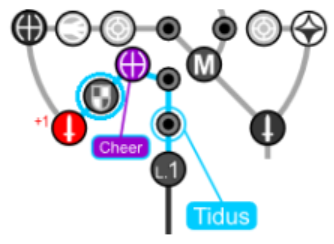
\includegraphics{graphics/tiduscheer}
	\end{itemize}
\end{spheregrid}
\begin{battle}[750]{Kimahri}
\begin{itemize}
	\tidusf Attack x3-7, depending on crits/Strength node.
\end{itemize}
\end{battle}
\begin{enumerate}[resume]
	\item \sd, continue running
\end{enumerate}
\begin{battle}{Garuda}
	\begin{itemize}
		\summon{\valefor}
		\valeforf Fire x6 to build \od
	\end{itemize}
\end{battle}
\begin{enumerate}[resume]
	\item If you didn't do the sphere grid yet, do it now.
	\item \formation{\tidus}{\yuna}{\lulu}
\end{enumerate}
\begin{battle}{Garuda}
	\begin{itemize}
		\item Flee using the Escape Command
	\end{itemize}
\end{battle}
\begin{encounters}
	\begin{itemize}
		\item Dingo: \tidus\ Attack
		\item Condor: \wakka\ Attack
		\item Water Flan: \lulu\ Thunder
	\end{itemize}
\end{encounters}
\begin{enumerate}[resume]
	\item At Besaid Beach go onto the boat.
\end{enumerate}
\chapter{S.S. Liki}

\begin{enumerate}
	 \item \cs[2:00], walk up to \yuna, \sd, walk back to \wakka, \sd, walk back up to \yuna, \cs + 4 \skippablefmv[4:20], \sd\ from `Sin!'
\end{enumerate}
\begin{battle}[2000]{Sin Fin}
	\begin{itemize}
		 \tidusf Defend
		 \switch{\yuna}{\lulu}
		 \luluf Thunder the Sin Fin
		 \kimahrif Lancet the Sin Fin
		 \enemyf Moves
		 \tidusf Defend
		 \kimahrif Lancet the Sin Fin
		 \luluf Thunder the Sin Fin
		 \switch{\tidus}{\yuna}
		 \summon{\valefor}
		 \valeforf Energy Blast \od\ on Sin Fin
	\end{itemize}
\end{battle}
\begin{enumerate}[resume]
	 \item \fmv+\cs[1:40]
\end{enumerate}
\begin{battle}[2000]{Sinspawn Echuilles}
	\begin{itemize}
		 \tidusf Cheer x2
		 \wakkaf Dark Attack
		 \tidusf Attack x2
		 \wakkaf Attack x2
		 \enemyf Blender
		 \wakkaf Attack x2
		 \tidusf Attack x2, one less if either \tidus\ crits or \wakka\ crits twice.
		 \tidusf \od
	\end{itemize}
	Check for \textbf{Ice Brand, Ice Ball}
\end{battle}
\begin{enumerate}[resume]
	\item \skippablefmv+\cs[1:30], \sd\ during \tidus\ monologue.
\end{enumerate}
\chapter{Kilika}

\begin{enumerate}
	\item \sd\ on exiting the boat, go up and left, \sd. \skippablefmv[2:00], (press Start immediately after skip) \sd
	\item Exit inn, go right to \wakka, \sd. Go left and up to Kilika Woods, \sd
\end{enumerate}
\begin{battle}{Lancet Tutorial}
	\begin{itemize}
		\item \sd
		\kimahrif Lancet
		\tidusf Attack
		\switch{anyone}{\yuna}
		\summon{\valefor}
		\valeforf Boost x2
		\valeforf Fire
	\end{itemize}
\end{battle}
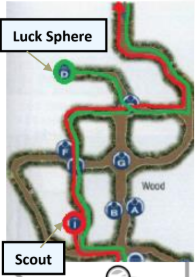
\includegraphics{graphics/kilikamap}
\begin{enumerate}[resume]
	\item Go left and up the hidden pack, \pickup{Scout Ball}
\end{enumerate}
\begin{spheregrid}
	\begin{itemize}
		\tidusf Go to Flee, learn Flee and Agility +1
	\end{itemize}
	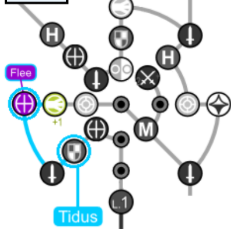
\includegraphics{graphics/tidusflee}
\end{spheregrid}
\begin{equip}
	\begin{itemize}
		\wakkaf Scout Ball
		\item \textit{If you got the Ice Brand:}
		\begin{itemize}
			\tidusf Ice Brand
		\end{itemize}
	\end{itemize}
\end{equip}
\begin{enumerate}[resume]
	\item \formation{\tidus}{\yuna}{\wakka}
	\item Continue up the hidden path, following the map.
\end{enumerate}
\begin{encounters}
	\begin{itemize}
		\item Killer Bee:
			\begin{itemize}
				\wakkaf Attack
				\luluf Blizzard
			\end{itemize}
		\item Dinonix: \tidus\ Attack
		\item Yellow Element: \lulu\ Water
		\item Ragora: Flee
	\end{itemize}
	Keep track of Speed Spheres, need 17 over the course of the run. Need about 45-55 AP on \tidus, which is about 6 kills these encounters.
\end{encounters}
\begin{enumerate}[resume]
	\item \sd
	\item \formation{\tidus}{\yuna}{\wakka}
	\item \save
\end{enumerate}
\begin{battle}[3000]{Sinspawn Geneaux}
	\begin{itemize}
	\item \textit{If \tidus\ is going before \yuna:}
	\begin{itemize}
		\tidusf Attack Main Body
		\summon{\valefor}
		\valeforf Energy Blast \od
		\valeforf Fire x4-5
	\end{itemize}
	\item \textit{Else:}
	\begin{itemize}
		\switch{\yuna}{\kimahri}
		\kimahrif Defend
		\tidusf Attack Main Body
		\switch{anyone}{\yuna}
		\summon{\valefor}
		\valeforf Energy Blast \od
		\valeforf Fire x4-5
	\end{itemize}
	\end{itemize}
\end{battle}
\begin{enumerate}[resume]
	\item \sd\ on stone steps and temple. go into temple. Walk up to \wakka\ and Pray. \sd\ inside temple and go up steps. Wait for life and \sd.
\end{enumerate}
\begin{trial}
	\begin{itemize}
		\item Take the sphere from the pedestal
		\item Place into the door, take it off of the door.
		\item Place sphere into the next door, take the sphere back.
		\item Place the sphere into the right holder
		\item Touch glpyh
		\item Take the sphere from the next room
		\item Place it into the left holder
		\item Take the glyphs sphere
		\item Place it in the Fire Room
		\item Take the sphere that you put into the right holder
		\item Use it to open the door in the Fire Room
		\item Take the sphere off the door
		\item Enter the Fayth room
	\end{itemize}
\end{trial}
\begin{enumerate}[resume]
	\item In Fayth room, \sd, speak to \wakka\ first. Try to leave room, \sd, name \ifrit
	\item Hold down to exit temple, \cs[0:40], \sd
	\item Go south through Kilika Woods, take the left path and \pickup{Luck Sphere}, referencing map.
	\item Exit Kilika Woods same way that you entered, treating fights the same way as above.
	\item Go down and right to S.S. Winno. \sd
\end{enumerate}
	
\chapter{S.S. Winno}
\begin{enumerate}
	\item \cs[1:10], exit door on the right. \sd\ with Oaka, then give him 1100 Gil. Run outside, go up to the top deck for \wakka\ and \lulu\ cutscene, \sd
	\item Run up the blitzball on the front of the boat. \cs[1:10]
	\item Follow the tutorial, fail the minigame
	\item \sd\ on \yuna's scene, do not save. \skippablefmv[0:30] if you buffered the Start command in Killika.
\end{enumerate}
\chapter{Luca}

\begin{enumerate}
	\item \sd, go right and up to the next screen, \cs[2:30]. Don't save.
	\item \sd\ in locker room. Don't do the tutorial. \sd, walk down, \sd
	\item Walk down to next screen, \sd. Whistle \cs[0:30], walk right to next screen.
	\item \sd, run to the cafe. \sd, \skippablefmv+\cs[1:20], \sd
	\item Run left ot next screen, then left to the docks. Run north to the next screen.
\end{enumerate}
\begin{battle}{Machina}
	\begin{itemize}
	\item \textit{For the first two encounters:}
	\begin{itemize}
		\tidusf Defend
		\kimahrif Defend
		\luluf Thunder
	\end{itemize}
	\item \textit{For the third encounter:}
	\begin{itemize}
		\item \textit{First Wave}
		\begin{itemize}
			\tidusf Attack
			\kimahrif Attack
			\luluf Thunder a different Machina
			\tidusf Attack
			\kimahrif \od\ Seed Cannon
		\end{itemize}
		\item \textit{Second Wave}
		\begin{itemize}
			\tidusf Defend
			\kimahrif Defend
			\luluf Thunder
		\end{itemize}
		\item \textit{Third Wave}
		\begin{itemize}
			\tidusf Attack
			\kimahrif Attack
			\luluf Thunder a different Machina
		\end{itemize}
	\end{itemize}
	\end{itemize}
\end{battle}
\begin{enumerate}[resume]
	\item If anyone is Critical HP, use Potions.
	\item Run right.
\end{enumerate}
\begin{battle}[3000]{Oblitzerator}
\begin{itemize}
	\kimahrif Defend
	\tidusf Defend
	\luluf Thunder Crane x3
	\tidusf Use Crane after \lulu's string
	\kimahrif Defend
	\luluf Thunder
	\tidusf Defend
\end{itemize}
Check for \textbf{Lightning Steel, Thunder Ball}
\end{battle}
\begin{enumerate}[resume]
	\item \cs[2:00], \sd\ during and after Blitzball game.
\end{enumerate}
\vfill
\begin{spheregrid}
	\begin{itemize}
		\tidusf Jump straight to Str Node
		\tidusf +1 Str, Haste, +20 MP
	\end{itemize}
	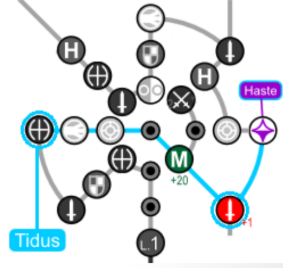
\includegraphics{graphics/haste}
\end{spheregrid}
\begin{equip}
	\begin{itemize}
		\item \textit{If you got Lightning Steel}
		\begin{itemize}
			\tidusf Equip Lightning Steel
		\end{itemize}
	\end{itemize}
\end{equip}
\begin{enumerate}[resume]
	\item Auto-Sort items
	\item Run South for the next two screens. \save. Go up the stairs to the locker room, \sd
	\item Go back into locker room, speak to \wakka, \sd, \cs[1:20]. \sd\ after \lulu\ scene. \cs[1:40] on Auron Entrance.
\end{enumerate}
\begin{trial}
	\textbf{Blitzball}
	\begin{itemize}
		\item \textit{If Luca wins the Blitzoff:}
		\begin{itemize}
			\item Triangle, switch the mode to \textbf{Mark Mode}
			\item When Graav is close to your central player, return to \textbf{Normal Mode}
		\end{itemize}
		\item \textit{When you get the ball:}
		\begin{itemize}
			\item Change to \textbf{Manual A} and \textbf{Normal Mode}
			\item Hide behidn the Goalie
			\item Alternatively pass to Jassu and swim around
			\item Only try to score when the time is almost up
			\item If losing, don't try to score
		\end{itemize}
		\item \sd\ during half time, \sd\ during \wakka\ protest, \sd\ end of game.
	\end{itemize}
\end{trial}
\begin{enumerate}[resume]
	\item \cs[1:00], Don't Save
\end{enumerate}
\begin{battle}{Sahagin Chief}
	\begin{itemize}
		\item{If no Lightning Steel:}
		\begin{itemize}
			\tidusf Haste \tidus
			\wakkaf Attack one Sahagin for the first two waves, defend on the third wave
			\tidusf Attack the other Sahagin
			\wakkaf Potion if \tidus\ has less than 150 HP
		\end{itemize}
		\item{If Lightning Steel:}
		\begin{itemize}
			\tidusf Cheer x2
			\wakkaf Attack
			\tidusf Attack
		\end{itemize}
	\end{itemize}
\end{battle}
\begin{enumerate}[resume]
	\item \sd
\end{enumerate}
\begin{battle}[1800]{Garuda}
	\begin{itemize}
		\tidusf Haste \auron
		\auronf Attack x3
		\wakkaf Defend
		\tidusf Defend until \auron\ finishes his string, then Attack
		\auronf Attack x3
		\item Don't revive non-\auron party members
	\end{itemize}
\end{battle}
\begin{enumerate}[resume]
	\item \cs+\skippablefmv[1:30]. Don't save. \sd\ the Auroch scene
	\item \cs[4:50]. Run north to the hidden chests, \pickup{Magic and HP Sphere}
	\item Run South and try to speak to \auron\ while he's walking away.
	\item Follow red arrow to \yuna. \sd\ during guardian scene. Walk to \yuna, \cs[4:20]
\end{enumerate}
\chapter{Mi'ihen Highroad}

\begin{enumerate}
	\item Walk up. Forced encounter, \sd. Walk up, \sd\ during Maechen Scene.
\end{enumerate}
\begin{encounters}
	\begin{itemize}
		\item Bomb:
		\begin{itemize}
			\switch{anyone}{\kimahri}
			\kimahrif Lancet Bomb, learn \textbf{Self Destruct}
			\item Flee.
		\end{itemize}
		\item Else Flee,  Heal afterwards if it was an ambush.
	\end{itemize}
\end{encounters}
\begin{enumerate}[resume]
	\item {Mi'ihen Skip}
	\begin{itemize}
		\item After Maechen Scene, run up as quickly as possible.
		\item Go to the White Spot on the ground towards the left before the Man in Blue
		\item Speak to the man, get the \textbf{Hunter's Spear}
		\item Mash and step forward over the cutscene line
		\item Walk up during the cutscene to the next screen.
	\end{itemize}
	\item Make sure you get the \textbf{Hunter's Spear} if you fail the skip.
	\item Go right and \sd\ at Calli scene. Continue walking up. \sd\ Luzzu scene, \sd\ Shelinda scene
	\item \formation{\tidus}{\yuna}{\auron}
	\item Go to the next screen
	\item Go to the Al-Bhed shop, \sd. Walk out of the shop and \cs[5:30]
	\item Leave shop, \sd. \sd\ on Rin. Walk outside.
\end{enumerate}
\begin{battle}{Chocobo Eater}
	\begin{itemize}
		\tidusf Haste Boss
		\tidusf Defend
		\auronf Defend
		\yunaf Attack \yuna\ to build \od
	\end{itemize}
\end{battle}
\begin{enumerate}[resume]
	\item \sd
	\item Walk north, \save. Walk north to next screen. Walk to blocked road, \sd. Speak to the guard on the right, \sd, walk back, \sd. Walk up to next screen.
\end{enumerate}
\chapter{Mushroom Rock Road}

\begin{enumerate}
	\item \sd, \cs. Walk back to guard to get \textbf{Tough Bangle}. Walk up, \sd, \sd.
	\item \textit{If you don't have \textbf{Self Destruct}, make sure that you get it before leaving the screen.}
	\item Flee from any encounters, go to the next screen.
	\item \save, go up the lift. Follow path.
	\item \formation{\tidus}{\wakka}{\auron}
\end{enumerate}
\begin{battle}{Non-Garuda Non-Ambush Anything}
	\begin{itemize}
		\switch{\tidus}{\kimahri}
		\kimahrif Defend
		\wakkaf Defend
		\switch{\auron}{\yuna}
		\summon{\valefor}
		\valeforf Energy Ray
	\end{itemize}
\end{battle}
\begin{enumerate}[resume]
	\item \formation{\tidus}{\wakka}{\auron}
\end{enumerate}
\vfill
\begin{spheregrid}
	\begin{itemize}
	\yunaf
	\begin{itemize}
		\item Use Magic Sphere
		\item +4 Magic
		\item Move to the right to +3 MagDef
		\item +3 MagDef, +3 Magic, +20 MP
		\item Move to Agil Node
		\item +3 Magic
	\end{itemize}
	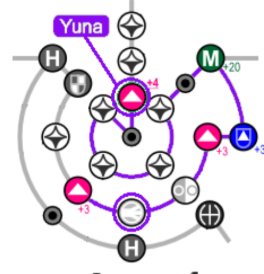
\includegraphics{graphics/yunammr}
	\kimahrif
	\begin{itemize}
		\item Move one right
		\item +200 HP
		\item Return to Lancet
		\item +200 HP
		\item Move to Agil node on the left
		\item +200 HP
	\end{itemize}
	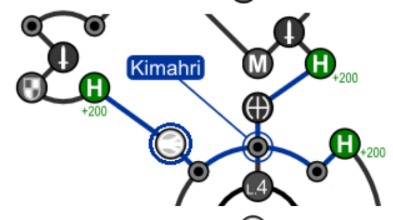
\includegraphics{graphics/kimahrimmr}
	\wakkaf
	\begin{itemize}
		\item Move to the HP node on the right
		\item +200 HP
		\item Move to Silence Attack on the right
		\item +2 Strength
	\end{itemize}
	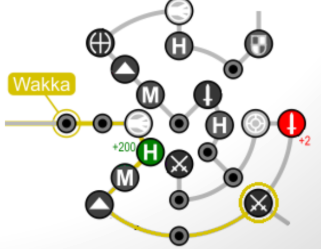
\includegraphics{graphics/wakkammr}
	\end{itemize}
\end{spheregrid}

\begin{encounters}
	\begin{itemize} % this can all be simplified down
		\item Raptor, Red Element, Gandarewa:
		\begin{itemize}
			\wakkaf Attack Raptor
			\switch{anyone}{\kimahri}
			\kimahrif Defend
			\switch{anyone}{\yuna}
			\summon{\valefor}
			\valeforf Boost
			\valeforf Blizzard Red Elemental
		\end{itemize}
		\item Raptor, Red Element, Fungar:
		\begin{itemize}
			\wakkaf Attack Raptor
			\switch{anyone}{\kimahri}
			\kimahrif Defend
			\switch{anyone}{\yuna}
			\summon{\valefor}
			\valeforf Fire Fungar
			\valeforf Boost
			\valeforf Blizzard Red Elemental
		\end{itemize}
		\item Raptor, Red Element, Lamashu:
		\begin{itemize}
			\wakkaf Attack Raptor
			\switch{anyone}{\kimahri}
			\kimahrif Attack Lamashtu
			\switch{anyone}{\yuna}
			\summon{\valefor}
			\valeforf Fire Lamashtu
			\valeforf Boost
			\valeforf Blizzard Red Elemental
		\end{itemize}
		\item Funguar, Red Element, Gandarewa:
		\begin{itemize}
			\wakkaf Attack Gandarewa
			\switch{anyone}{\kimahri}
			\kimahrif Defend
			\switch{anyone}{\yuna}
			\summon{\valefor}
			\valeforf Fire Funguar
			\valeforf Boost
			\valeforf Blizzard Red Elemental
		\end{itemize}
		\item Raptor, Red Element, Gandarewa:
		\begin{itemize}
			\wakkaf Attack Gandarewa
			\switch{anyone}{\kimahri}
			\kimahrif Attack Lamashtu
			\switch{anyone}{\yuna}
			\summon{\valefor}
			\valeforf Fire Lamashtu
			\valeforf Boost
			\valeforf Blizzard Red Elemental
		\end{itemize}
	\item Garuda: Flee
	\end{itemize}
\end{encounters}
\begin{enumerate}[resume]
	\item While Yuna still needs AP, do the following
\end{enumerate}
\begin{encounters}
	\begin{itemize}
		\wakkaf Attack Raptors or Gandarewas
		\switch{anyone}{\yuna}
		\yunaf Defend
		\item Flee
	\end{itemize}
\end{encounters}
\begin{enumerate}[resume]
	\item Make sure that you've completed the above sphere grid.
	\item \formation{\tidus}{\yuna}{\wakka}
	\item Go on lift, go to HQ. Go onto the main lift andonto the next screen.
	\item Walk down and \sd. Walk right to next screen, then right, \sd. Walk right to Oaka
\end{enumerate}
\begin{shop}{10890}
	\begin{itemize}
	\item Sell
	\begin{itemize}
		\item Hi-Potions
		\item Elixers
		\item Tough Bangle
		\item Hunter's Spear
	\end{itemize}
	\item Buy
	\begin{itemize}
		\item Sentry, Equip
	\end{itemize}
	\end{itemize}
\end{shop}
\begin{enumerate}[resume]
	\item \sd, go right, \cs[1:00], \sd\ after Seymour. Go down to guard, confirm Yes, \sd
\end{enumerate}
\begin{battle}[12000]{Sinspawn Gui1}
\begin{itemize}
	\tidusf Defend
	\switch{\yuna}{\auron}
	\auronf Power Brain Main Body
	\wakkaf Switch Weapon, to Thunder Ball, otherwise to same.
	\switch{\wakka}{\kimahri}
	\kimahrif Self Destruct main body
	\switch{\tidus}{\yuna}
	\summon{\valefor}
	\valeforf Energy Blast \od\ x2
\end{itemize}
\end{battle}
\begin{enumerate}[resume]
	\item \cs+\skippablefmv[2:20]. \sd\ Seymour dialogue.
\end{enumerate}
\begin{battle}[6000]{Sinspawn Gui 2}
\begin{itemize}
	\item \textbf{\textcolor{YellowGreen}{Seymour}}: Fira Head
	\item \textbf{\textcolor{YellowGreen}{Seymour}}: Fira Body x6
	\yunaf Defend
	\auronf Defend
\end{itemize}
\end{battle}
\begin{enumerate}[resume]
	\item \sd, \cs+\skippablefmv[2:00], walk left and up to Gatta, \sd. \fmv+\cs[1:30], \sd\ during \tidus\ monologue. \cs[1:00], \sd
	\item Walk left, \sd. Walk left, speak to \auron, \sd. Go up and right, \sd, exit area, \sd.
\end{enumerate}
\vfill
\ 
\columnbreak


\chapter{Djose}

\begin{spheregrid}
\begin{itemize}
	\tidusf
	\begin{itemize}
		\item Go up to Str +1
		\item Str+1, HP+200, Agil+2
	\end{itemize}
	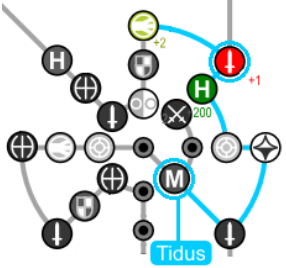
\includegraphics{graphics/djosetidus}
	\wakkaf
	\begin{itemize}
		\item Go up to HP Node
		\item Str +2
		\item Return to Silence Attack
	\end{itemize}
	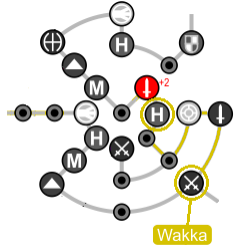
\includegraphics{graphics/djosewakka}
\end{itemize}
\end{spheregrid}
\begin{enumerate}
	\item \formation{\tidus}{\yuna}{\auron}
	\item Walk North.
\end{enumerate}
\begin{encounters}
	\begin{itemize}
		\item Basilisk:
		\begin{itemize}
			\switch{anyone}{\kimahri}
			\kimahrif Lancet Basilisk, learn \textbf{Stone Breath}
			\item Flee.
		\end{itemize}
		\item Else Flee,  Heal afterwards if it was an ambush.
	\end{itemize}
\end{encounters}
\begin{enumerate}[resume]
	\item Continue walking north, \sd, walk up to the next screen.
	\item Walk along brdige to next screen, \sd, walk into temple. Speak to \auron\ at the doorway, \sd, walk up the stairs.
\end{enumerate}
\vfill
\begin{trial}
\begin{itemize}
	\item Take the sphere from the left wall
	\item Place into door
	\item Take the sphere from the right wall
	\item Place into door
	\item Take the sphere from the left wall
	\item Push pedestal to the right
	\item Put sphere into wall
	\item Take right sphere
	\item Place into far right wall
	\item \cs
	\item Take spher from left wall
	\item Reset puzzle in the far left tile
	\item Place sphere into pedestal
	\item Take the pedestal sphere
	\item Put sphere into right wall
	\item Take the far right sphere
	\item Put into pedestal
	\item Push pedestal through the door
	\item Jump onto pedestal
	\item Push the second pedestal, return to main room
	\item Place charged sphere into the left wall
	\item Reset
	\item Place the two pedestal spheres in the first left and right walls
	\item Go onto the lift in the center
	\item Push all the pedestals in, walk up the stairs
\end{itemize}
\end{trial}
\begin{enumerate}[resume]
	\item Talk to \auron, wait. \sd, try to leave, \sd, name \ixilon
	\item Speak to \auron, enter the temple and go ot the left room. Speak to the priest, \sd. Exit the temple, \sd
	\item Go left, \pickup{4000 Gil}, cross the bridge, \sd, exit, \sd, go up to Moonflow.
\end{enumerate}
\chapter{Moonflow}

\begin{enumerate}
	\item Walk north, \sd\ on Kimahri Scene.
	\item Near the end of the screen, go left through the hidden path. \pickup{Magic Def Sphere}
	\item Walk north, \sd, walk lef,t \sd, walk left past 2 screens, \sd. Walk right and ride ze shoopuf, \sd.
\end{enumerate}
\begin{battle}[4000]{Extractor}
\begin{itemize}
	\tidusf Haste self, then \wakka
	\wakkaf Attack
	\textit{If Lightning Steel:}
	\begin{itemize}
		\item Cheer x1
	\end{itemize}
	\textit{Else:}
	\begin{itemize}
		\item \textit{If Tidus went First} Cheer x4 
		\item \textit{If Tidus went Second} Cheer x5
	\end{itemize}
	\tidusf Attack
\end{itemize}
\end{battle}
\begin{enumerate}[resume]
	\item \sd, walk left to next screen, walk left and talk to \rikku, \sd
	\item Walk up to the forced encounter
\end{enumerate}
\begin{battle}{Rikku Tutorial}
\begin{itemize}
	\item Complete tutorial
	\rikkuf Mix 2 Potions for the \od
	\item Flee
\end{itemize}
\end{battle}
\begin{enumerate}[resume]
	\item Walk to next screen.
	\item \formation{\tidus}{\yuna}{\auron}
	\item Heal everyone with Potions
	\item Walk north to next screen.
\end{enumerate}
\chapter{Guadosalam}

\begin{enumerate}
	\item \sd, walk to Seymour's house, try to leave. Walk into room, speak to \auron, \sd, speak to \lulu, \wakka, \rikku, \yuna. \sd, \fmv+\cs[5:50]
	\item Exit the house, walk down, \sd. Go to the Farplane. Hidden in the screen goign to the Farplane, \pickup{Lightning Marble x8}
	\item \sd, speak to \auron, go into the Farplane. \cs[1:20]. Speak to \wakka, \sd, speak to \yuna, \cs[2:10], \sd.
	\item Go to Seymour House Entrance, \sd
	\item Guadosalam Skip:
	\begin{itemize}
		\item Stand outside of the Potion Shop
		\item Wait until you get pushed by the Guado to trigger the skip
		\item Run to the exit using the minimap
		\item If on HD Remaster, speak to the woman on the left to stop her walking abit, then speak to the running Guado as the woman pushes you to into the door.
	\end{itemize}
	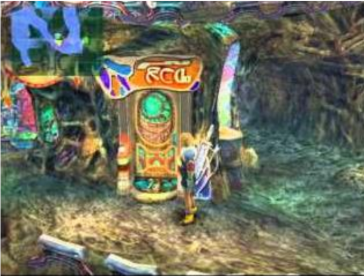
\includegraphics{graphics/guadoskipstandard}

	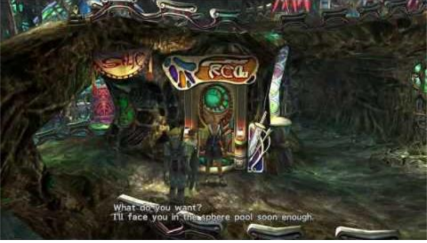
\includegraphics{graphics/guadoskipremaster}
\end{enumerate}
\chapter{Thunder Plains}

\begin{enumerate}
	\item \formation{\tidus}{\rikku}{\auron}
	\item Walk north, dodging lightning. Make sure that you end Thunder Planes with the Light Curtain.
\end{enumerate}
\begin{encounters}
\begin{itemize}
	\item Melusine: Steal for Petrify Grenade, Flee
	\item Buer: If short of Speed Spheres, can throw Grenades
	\item Iron Giant:
	\begin{itemize}
		\switch{anyone}{\yuna}
		\yunaf Attack to build \od
		\rikkuf Steal Light Curtain
		\item Flee
	\end{itemize}
	\item Larva: If Blitz Loss, steal Lunar Curtain
\end{itemize}
\end{encounters}
\begin{enumerate}[resume]
	\item \sd\ when approaching Al Bhed shop. Walk into the shop when \rikku begs to go inside.
\end{enumerate}
\begin{shop}{???}
\begin{itemize}
	\item Sell: Longsword
	\item \textit{Blitz Loss:}
	\begin{itemize}
		\item Sell: Other Equipment worth 1k+ Gil
		\item Buy: Baroque Sword
	\end{itemize}
	\item Buy:
	\begin{itemize}
		\item Shimmering Blade
		\item 14 Phoenix Downs
		\item 3 Grenades, +1 for every Buer encounter you want for Speed Spheres
	\end{itemize}
\end{itemize}
\end{shop}
\begin{enumerate}[resume]
	\item Walk into shop corridor, \cs[2:00]
	\item Speak to \auron, then to \rikku, \sd.
	\item Pickup the \textbf{Yellow Shield} outside the shop on the ground.
	\item Exit screen, go north, near the exit \sd, \cs[3:10]
\end{enumerate}
\chapter{Macalania Woods}

\begin{enumerate}
	\item \sd, walk north, \sd, \save
	\item \formation{\tidus}{\rikku}{\auron}
	\item Follow path, \pickup{2000 Gil}
	\item Make sure that you build up \rikku\ \od, and that you do at least one of each of the following steals.
\end{enumerate}
\begin{encounters}
\begin{itemize}
	\item Chimera: Steal Arctic Wind, Flee
	\item Blue Elementa: Steal Fish Scale x2, Flee
	\item Else: Flee
\end{itemize}
\end{encounters}
\begin{enumerate}[resume]
	\item Follow path, \sd\ twice
	\item On the final screen, hidden behind the tree, \pickup{Remedy}
	\item Catch butterfly near the exit to avoid encounters
	\formation{\tidus}{\yuna}{\kimahri}
	\item \save, talk to Oaka. Say his ``Prices are too expensive'', go in again.
\end{enumerate}
\begin{shop}{???}
\begin{itemize}
	\item Buy: Sonic Steel, Equip
\end{itemize}
\end{shop}
\begin{enumerate}[resume]
	\item Run up, \sd. Enter the hidden path, walk to \auron, \sd
\end{enumerate}
\begin{battle}[12000]{Spherimorph}
\begin{itemize}
	\tidusf Change Armor to Yellow Shield
	\tidusf Defend
	\switch{\tidus}{\rikku}
	\rikkuf Granade, check the Element
	\kimahrif Defend
	\yunaf Defend
	\rikkuf \od, Mag Def Sphere with
	\begin{itemize}
		\item Fire: Arctic Wind
		\item Ice: Bomb Core
		\item Water: Lightning Marble
		\item Thunder: Fish Scale
	\end{itemize}
\end{itemize}
\end{battle}
\begin{enumerate}[resume]
	\item \cs[1:50], \sd, \sd
	\item Auto Sort Items, put Phoenix Downs in the First Slot and Lightning Marbles in the Third
\end{enumerate}
\begin{spheregrid}
\begin{itemize}
	\rikkuf
	\begin{itemize}
		\item Move down 2 nodes (1 if you're doing quick hit)
		\item Agi+3
	\end{itemize}
	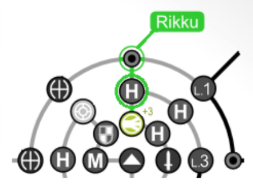
\includegraphics{graphics/macalaniarikku}
	\kimahrif
	\begin{itemize}
		\item Move to the bottom left of the grid
		\item Agi+3, Level 1 Key Sphere
		\item Move further left
		\item Level 1 Key Sphere
		\item Go to Steal Node
		\item Steal, Use
	\end{itemize}
	\yunaf
	\begin{itemize}
		\item Agi +3, HP +200, Def +2
		\item Level 2 Key Sphere
		\item Str + HP Nodes
		\item Agi+2 Node
		\item Stop at Str +4
		\item Can this please be more specific
	\end{itemize}
\end{itemize}
\end{spheregrid}
\begin{enumerate}[resume]
	\item Heal Party, with Cure/Mega-Potions
	\item \formation{\tidus}{\lulu}{\kimahri}
	\item Talk to \auron\ on the way out, then exit
\end{enumerate}
\vfill \ 
\newpage

\chapter{Lake Macalania}

\begin{enumerate}
	\item Run up and \sd
\end{enumerate}
\begin{battle}[1600]{Crawler}
\begin{itemize}
	\switch{\tidus}{\rikku}
	\rikkuf Lightning Marble x2/3 Crawler
	\kimahrif Lightning Marble Crawler
	\enemyf Assault \rikku
	\luluf Phoenix Down \rikku
	\switch{\kimahri}{\yuna}
	\yunaf Defend
	\rikkuf Lightning Marble Crawler
	\enemyf Assault \rikku
	\switch{\yuna}{\tidus}
	\tidusf Defend
	\rikkuf \od, HP Sphere and Lightning Marble
\end{itemize}
\end{battle}
\begin{spheregrid}
\begin{itemize}
	\tidusf
	\begin{itemize}
		\item Level 2 Key Sphere
		\item Move to Mental Break
		\item Str +4
		\item Move to Evasion
		\item HP+200
		\item Move to HP+200 Node
		\item HP+200, Str+4, Agi+2
		\item Move right one node
		\item Use Strength Sphere, Activate it
		\item Move to Central Agility Node
		\item HP+200, Str+4, Agi+2
		\item Move Left
		\item Str+4
		\item Tidus should have 1320 Max HP
	\end{itemize}
\end{itemize}
\end{spheregrid}
\begin{enumerate}[resume]
	\item \sd, \cs[0:40], head to next screen
	\item Head to Temple, \sd. \save, speak to Tromell for \textbf{Shell Target}
	\item Jyscal Skip:
	\begin{itemize}
		\item Walk into the wall to the right of Tromell
		\item Move slightly to the right, turn around and Talk to Tromell while moving Right.
		\item If successful, walk forward whil emashing Shelinda's dialogue.
		\item When done, walk up the stairs and push the man and go through.
		\item If Shelinda is not saying her dialogue, talk to one of the musicians
	\end{itemize}
	\item \sd, walk to Fayth room, \cs[2:10]
\end{enumerate}
\vfill
\begin{battle}[3000]{Seymour}
\begin{itemize}
	\tidusf Switch to Brotherhood
	\tidusf Haste \tidus
	\enemyf Seymour Blizzara
	\yunaf Change Weapon Staff to Staff
	\enemyf Guado Guardians None/Blizzard/Thunder/Shremedy
	\kimahrif Defend. If Shremedy landed, Remedy/Attack the afflicted target. If \yuna\ is dead, Phoenix Down
	\switch{\yuna}{\auron}
	\auronf Defend
	\tidusf \od\ Spiral Cut Seymour
\end{itemize}
\end{battle}
\begin{battle}[18000]{Anima}
\begin{itemize}
	\switch{\tidus}{\wakka}
	\wakkaf Change Weapon
	\item \textit{If you lost Blitz:}
	\begin{itemize}
		\kimahrif Lightning Gem/Bomb Core/Arctic Wind
	\end{itemize}
	\item \textit{Else:}
	\begin{itemize}
		\kimahrif Steal
	\end{itemize}
	\enemyf Pain
	\switch{first survivor}{\tidus}
	\tidusf Attack x4
	\switch{second survivor}{\rikku}
	\rikkuf Steal
	\rikkuf Phoenix Down \yuna\ if she's dead
	\rikkuf \textit{Blitz Loss:} Use lightning Gem/Bomb Core/Arctic Wind
\end{itemize}
\end{battle}
\begin{battle}[6000]{Seymour}
\begin{itemize}
	\tidusf Swap Weapon to \textbf{Sonic Steel}
	\tidusf Attack x2/3
	\rikkuf \textit{On Blitz Win:} Phoenix Down Lulu
	\rikkuf Defend
\end{itemize}
\end{battle}
\begin{enumerate}[resume]
	\item Name \shiva, \save, exit Fayth room.
\end{enumerate}
\begin{trial}
\begin{itemize}
	\item Slide pedestal to the right
	\item Take sphere from the right, place into pedestal
	\item Push pedestal up
	\item Take Glyphs sphere from wall, go downstairs.
	\item Place Glyphs sphere in left wall
	\item Go upstairs, pick up sphere
	\item Go downstairs, place sphere in pillar
	\item Go upstairs, take the last sphere
	\item Place in pillar
\end{itemize}
\end{trial}
\begin{spheregrid}
\begin{itemize}
	\tidusf
	\begin{itemize}
		\item Move Left
		\item HP+200, Str+4, Agi+2
	\end{itemize}
\end{itemize}
\end{spheregrid}
\begin{enumerate}[resume]
	\item Equip Sonic Steel if not done
	\item \formation{\tidus}{\rikku}{\yuna}
	\item Go to temple entrance, \sd
	\item Move south and go down the left path.
	\item If Blitz Loss, do one of the following encounters:
\end{enumerate}
\begin{encounters}
\begin{itemize}
	\item Guado Fight:
	\begin{itemize}
		\tidusf Attack
		\rikkuf Silence Grande
		\yunaf Defend
	\end{itemize}
\end{itemize}
\end{encounters}
\begin{battle}[18000]{Wendigo}
\begin{itemize}
	\tidusf Haste \tidus
	\tidusf Switch Weapon to Brotherhood
	\tidusf Attack Guado B
	\rikkuf Light Curtain \tidus
	\tidusf Attack Wendigo
	\yunaf Defend/Heal \tidus/Phoenix Down Dead Ally
	\rikkuf Defend/Heal \tidus/Steal Guado/Phoenix Down Dead Ally
	\item Make sure that \yuna survives in the end
\end{itemize}
\end{battle}
\begin{enumerate}[resume]
	\item Run up to \rikku, \sd, walk up to \yuna, \sd, \save, run past \kimahri\ and go to the hidden area to \pickup{Level 2 Key Sphere}
	\item Run up to \auron\ and speak with him, \sd, walk bac, \cs+\skippablefmv[1:00], \sd\ in Dream Sequence
\end{enumerate}


\chapter{Bikanel Desert}
\begin{spheregrid}
\begin{itemize}
	\tidusf Move down and activate Str+4
\end{itemize}
\end{spheregrid}
\begin{enumerate}
	\item You need 21 Power Spheres from now on
	\tidusf Equip Sonic Steel
	\item Walk up, \sd, \save, walk up
\end{enumerate}
\begin{battle}{Zu}
\begin{itemize}
	\tidusf Defend
	\tidusf Attack
	\tidusf Defend until all party members arrive
	\item Flee
\end{itemize}
\end{battle}
\begin{enumerate}[resume]
	\item \sd
	\item Run up to meet with \wakka, \sd. Go left to enter next screen, go right to join with \kimahri, \sd. Run back and then up to meet \rikku, \sd, \save
	\item \formation{\tidus}{\kimahri}{\auron}
	\item Heal everyone with a Mega-Potion
	\item Make sure that \rikku's \od\ is full and \tidus's is at least 75\%
	\item Continue along path. On the next screen, go in north-west towards the save sphere, take the shortcut to the left. Go up to the next screen and fight the Sandragora fights. They're located in the Top Right Sinkhole with Chest, and then at the end of the path up and to the left, then go up and \sd
	\item Ideally you want 6 total Sleeping Powders, Smoke Bombs, Silence GrandeGrenades
\end{enumerate}
\begin{encounters}
\begin{itemize}
	\item Sand Wolf: Steal Sleeping Powders, then Flee
	\item Zu: Steal Smoke Bomb x3, then Flee
	\item Alcyone: Steal Smoke Bomb, then Flee.
	\begin{itemize}
		\item If short on Speed Spheres, use the Smoke Bombs on them.
	\end{itemize}
	\item Otherwise: Flee
\end{itemize}
\end{encounters}
\begin{battle}{Sandragora 1}
\begin{itemize}
	\tidusf Haste \kimahri
	\kimahrif \od\ Stone Breath
\end{itemize}
\end{battle}
\begin{battle}{Sandragora 2}
\begin{itemize}
	\tidusf Haste \auron
	\auronf \od\ Shooting Star (Triangle, O, Square, X, $\leftarrow, \rightarrow$, X)
\end{itemize}
\end{battle}
\chapter{Home}

\begin{enumerate}
	\item \formation{\tidus}{\auron}{\lulu}
	\item Go into door, \sd
\end{enumerate}
\begin{battle}{Bombs}
\begin{itemize}
	\tidusf Haste \tidus
	\tidusf Attach each
	\auronf Attack whatever didn't die to \tidus
\end{itemize}
\end{battle}
\begin{enumerate}[resume]
	\item \sd
\end{enumerate}
\begin{battle}{Dual Horn}
\begin{itemize}
	\switch{anyone}{\kimahri}
	\kimahrif Lancet Chimera (Aqua Breath)
	\kimahrif \od\ Stone Breath
\end{itemize}
\end{battle}
\begin{enumerate}[resume]
	\item Restore party HP
	\item \textit{If you lost Blitz:}
	\begin{itemize}
		\item Go down the stairs. Once the camera flips, \formation{\tidus}{\auron}{\rikku}, go back up the stairs into the door.
		\item Do the following Dual Horn encounter

		\begin{battle}{Dual Horns - Blitz Loss}
		\begin{itemize}
			\tidusf Haste \tidus
			\tidusf Attack
			\rikkuf Petrify Grenade/Smoke Bomb
		\end{itemize}
		\end{battle}
		\item Open the following chests: Bottom Middle (up x2), Midle Right (up x3), Middle (down x4) %wtf does this line mean
	\end{itemize}
	\item Go down and left, \cs[0:50]
\end{enumerate}
\begin{battle}{Chimera}
\begin{itemize}
	\switch{anyone}{\kimahri}
	\kimahrif Lancet
	\kimahrif \od\ Stone Breath
\end{itemize}
\end{battle}
\begin{enumerate}[resume]
	\item Walk down steps, \cs[1:30]
	\item Before going further, \pickup{Level 2 Key Sphere}
	\item \sd\ until Tidus asks ``why'', \cs[6:20]
	\item Go bottom right to the next screen, run across the bridge
\end{enumerate}
\chapter{Airship}

\begin{enumerate}
	\item \sd\ during \cs+3 \skippablefmv. Walk down corridor to the next screen, go back in, \sd. Speak to Brother, \sd. Walk towards corridor, \sd. Walk towards camera to the next screen, go up and speak to Rin.
	\item If missing any spheres, buy Distillers from Rin. Each one counts as 2 Spheres.
	\item \save. Make sure that \rikku\ has \od
	\item \formation{\tidus}{\rikku}{\kimahri}
\end{enumerate}
\begin{battle}[32000]{Evrae}
	\begin{itemize}
	\item \textit{If you won Blitz:}
	\begin{itemize}
		\tidusf Haste \tidus
		\tidusf Cheer
		\tidusf If \tidus\ is still going next, Change Armor
		\rikkuf \od\ Mix Luck Sphere + Map
		\tidusf Attack x2
		\tidusf Cheer
		\tidusf Attack x3
		\kimahrif Heal \tidus\ if he was hit in the first attack, Steal otherwise
		\rikkuf Steal
	\end{itemize}
	\item \textit{If you lost Blitz:}
	\begin{itemize}
		\tidusf Haste \tidus
		\tidusf Cheer x2
		\tidusf Equip Baroque Sword
		\tidusf Attack x6
		\rikkuf \od\ Mix Luck Sphere + Map
		\item \kimahri\ or \rikku: Full Heal \tidus, Lunar Curtaion \tidus
		\item \kimahri\ or \rikku: Steal
	\end{itemize}
\end{itemize}
\end{battle}
\chapter{Bevelle}
\begin{enumerate}
	\item Use a Mega-Potion
	\item \textit{With Sleeping Powder:}
\end{enumerate}
\begin{battle}{Guard Fights - Sleeping Powder}
\begin{itemize}
	\item \textit{Fights 1 and 3:}
	\begin{itemize}
		\tidusf Attack
		\item Defend or use Distillers
	\end{itemize}
	\item \textit{Fights 2 and 4:}
	\begin{itemize}
		\tidusf Attack
		\rikkuf Sleeping Powder
		\kimahrif Silence Grenade/Smoke Bomb/Distiller
	\end{itemize}
	\item \textit{Fight 5:}
	\begin{itemize}
		\tidusf Haste \rikku
		\rikkuf Throw Items x2
		\tidusf Attack
	\end{itemize}
\end{itemize}
\end{battle}
\begin{enumerate}[resume]
	\item \textit{Without Sleeping Powder:}
	\item \formation{\tidus}{\rikku}{\auron} \textit{unless \lulu\ doesn't have at least 35 levels, then } \formation{\tidus}{\rikku}{\lulu}
\end{enumerate}
\begin{battle}{Guard Fights - No Sleeping Powder}
\begin{itemize}
	\item \textit{Fights 1 and 3:}
	\begin{itemize}
		\tidusf Attack
		\item Defend or use Distillers
	\end{itemize}
	\item \textit{Fights 2 and 4:}
	\begin{itemize}
		\switch{\tidus}{\kimahri}
		\kimahrif Silence Grenade/Smoke Bomb
		\switch{\rikku}{\tidus}
		\tidusf Attack
		\kimahrif Repeat
	\end{itemize}
	\item After the second fight, \formation{\tidus}{\rikku}{\lulu}
	\item \textit{Fight 5:}
	\begin{itemize}
		\switch{\tidus}{\rikku}
		\rikkuf Silence Grenade/Smoke Bomb x2
		\switch{\kimahri}{\tidus}
		\tidusf Attack
	\end{itemize}
\end{itemize}
\end{battle}
\begin{enumerate}[resume]
	\item \sd, \fmv[1:30], \sd\ on \yuna\ dialogue. \skippablefmv[30], \sd. Use lift, \sd.
\end{enumerate}
\begin{trial}
\begin{itemize}
	\item Push the pedestal in
	\item Press X
	\item Go left at the second junction
	\item Take sphere, push pedestal back into the junction
	\item At the third junction, go back
	\item Go left at the second junction
	\item Place sphere into wall, push pedestal back
	\item Go left at the first junction
	\item Go left
	\item At the third junction and go right
	\item Take glyph sphere from wall, push pedestal back onto the road
	\item At the fourth junction go right
	\item Place glyph sphere into pedestal
	\item Take Vevelle sphere from pedestal
	\item Place Bevelle sphere into the wall
	\item Take the glyph sphere
	\item Place into the next wall
	\item Take Destruction sphere from the new wall %where to put it
	\item Take Bevelle sphere from old wall
	\item Push pedestal back and fall off the edge
	\item Go straight
	\item At the third junction go right
	\item Place destruction sphere into wall
	\item Push pedestal back and fall off the edge
	\item Go straight
	\item At the second junction go right
	\item Push pedestal
	\item Go up the stairs, open the chest
\end{itemize}
\end{trial}
\begin{enumerate}[resume]
	\item \sd, name \bahamut, don't save, \sd
\end{enumerate}

\chapter{Via Prifico}

\begin{enumerate}
	\item Run up past the first telepad
	\item Go to the second telepad and travel north.
	\item When you get Auron:
\end{enumerate}
\begin{spheregrid}
\begin{itemize}
	\auronf
	\begin{itemize}
		\item Unlock both Leve 2 Key Sphere Nodes
		\item Move to Wakka's Grid
		\item Go Left to Emtpy Node adjacent to Mag +3, up x2 from where you unlocked the second Level 2 Node
		\item Mag+3
	\end{itemize}
	\yunaf
	\begin{itemize}
		\item Teleport Sphere to Auron's Magic Node
		\item Mag+3, Str+4
		\item Go right
		\item Get all Str, Hp, Mag, Def, Agi, MP nodes
		\item Stop on Silence Buster
	\end{itemize}
\end{itemize}
\end{spheregrid}
\begin{enumerate}[resume]
	\item Check how many Power Spheres you have left, you need 13 more for the rest of the run
	\item Keep track of how many things you kill here.
\end{enumerate}
\begin{encounters}
\begin{itemize}
	\item Maze Larva: Summon \ixilon, Attack
\end{itemize}
\end{encounters}
\begin{battle}{Isaaru}
\begin{itemize}
	\item Grothia (8000 HP):
	\begin{itemize}
		\summon{\bahamut}
		\bahamutf Attack
	\end{itemize}
	\item Pterya (12000 HP):
	\begin{itemize}
		\summon{\bahamut}
		\bahamutf Attack x2
	\end{itemize}
	\item Spathi (12000 HP):
	\begin{itemize}
		\summon{\ixilon}
		\ixilonf Attack x5
	\end{itemize}
\end{itemize}
\end{battle}
\begin{enumerate}[resume]
	\item Swim right and then up. If needed, you can attack Yellow Starfish with \tidus\ for 2x Power Spheres.
\end{enumerate}
\begin{battle}{Evrae Altana}
\begin{itemize}
	\item Anyone: Phoenix Down x2/Elixer Evrae Altana
\end{itemize}
\end{battle}
\begin{enumerate}[resume]
	\item Swim to exit, \sd
	\item Walk north
	\item From this point on, watch any pre-empts if \yuna\ is in the party, because she can get the first turn. Check to make sure that \lulu\ has 35 levels.
	\item \formation{\tidus}{\yuna}{\auron}
\end{enumerate}
\begin{spheregrid}
\begin{itemize}
	\yunaf
	\item \textit{If you won Blitz:}
	\begin{itemize}
		\item Teleport to Strength Sphere (Up x2)
		\item Str+4, Str+4
		\item Go left
		\item Str+4, Agi+2, Str+4
	\end{itemize}
	\item \textit{If you lost Blitz:}
	\begin{itemize}
		\item Teleport to Tidus Str+4 by Mental Break
		\item Str+4
		\item Friend Sphere to \tidus
		\item Proceed backwards through \auron's grid, grabbing all Str nodes and 1 Agi node
	\end{itemize}
\end{itemize}
\end{spheregrid}
\begin{encounters}
\begin{itemize}
	\item YKT-63 (get 4 kills):
	\begin{itemize}
		\tidusf Attack
		\yunaf Attack
		\item Flee
	\end{itemize}
\end{itemize}
\end{encounters}
\begin{spheregrid}
\begin{itemize}
	\yunaf
	\item \textit{If you won Blitz:}
	\begin{itemize}
		\item Move left
		\item Str+4
	\end{itemize}
	\item \textit{If you lost Blitz:}
	\begin{itemize}
		\item Move right
		\item Str+4
	\end{itemize}
\end{itemize}
\end{spheregrid}
		
\begin{battle}[36000]{Seymour Natus}
\begin{itemize}
	\item \textit{If \lulu\ has less than 35 levels:}
	\begin{itemize}
		\switch{\tidus}{\lulu}
		\luluf Switch Weapon
		\switch{\lulu}{\tidus}
	\end{itemize}
	\tidusf Attack
	\summon{\bahamut}
	\bahamutf Attack
\end{itemize}
\end{battle}
\begin{enumerate}[resume]
	\item \sd
\end{enumerate}
\begin{equip}
\begin{itemize}
	\tidusf Sonic Steel
	\auronf Shimmering Blade
\end{itemize}
\end{equip}
\begin{enumerate}[resume]
	\item Walk to \yuna, \cs+\skippablefmv[10:10]. Walk down, \cs[1:40], walk right, \save, exit Macalania Woods
\end{enumerate}	
\chapter{Calm Lands}

\begin{enumerate}
	\item \sd, walk left
	\item If you only have 1 \textbf{Water Gem}, steal a \textbf{Fire Gem} from one of the Flame Flans.
\end{enumerate}
\begin{spheregrid}
\begin{itemize}
	\yunaf Str+4
\end{itemize}
\end{spheregrid}
\begin{enumerate}[resume]
	\item \formation{\tidus}{\kimahri}{\yuna}
	\item Continue north to the Calm Lands Exit
	\item Run north, \sd
\end{enumerate}
\begin{battle}[64000]{Defender X}
\begin{itemize}
	\switch{\tidus}{\yuna}
	\summon{\bahamut}
	\bahamutf Attack x2
\end{itemize}
\end{battle}
\begin{enumerate}[resume]
	\item \sd, walk across bridge and up to Mt. Gagazet, \sd
\end{enumerate}
	
\chapter{Mt. Gagazet}
\begin{enumerate}
	\item Walk up, \cs[3:40], walk up, \sd
\end{enumerate}
\begin{battle}{Brian and Yenke}
\begin{itemize}
	\kimahrif Steal from Biran
	\item Gem Yenke
	\item Gem Biran
\end{itemize}
Pay attention to your drops
\end{battle}
\begin{enumerate}[resume]
	\item \formation{\tidus}{\kimahri}{\wakka}
	\item Make sure you charge \rikku's \od
\end{enumerate}
\begin{spheregrid}
\begin{itemize}
	\luluf Move up, unlock the Level 2 Key Sphere
	\begin{itemize}
		\item Move down, unlock the Level 3 Key Sphere to the left of Bribe
		\item Move to the first Str+4 node
	\end{itemize}
	\yunaf
	\begin{itemize}
		\item \textit{If you got \textbf{4 Return Spheres}:}
		\begin{itemize}
			\item Return to the last Str+2 node in \wakka's grid ($\downarrow \downarrow \rightarrow \rightarrow \downarrow \downarrow$)
			\item Move left
			\item Mag+3, Level 1 Key Sphere
			\item Move down
			\item Str+2, Agi+4
		\end{itemize}
		\item \textit{If you got \textbf{2 Return Spheres}:}
		\begin{itemize}
			\item Friend Sphere to \lulu
			\item Str+4, Str+4
			\luluf Go to Str+3
			\yunaf Friend Sphere to \lulu
			\item Str+3, Agi+4, Agi+4
		\end{itemize}
		\item \textit{If you got \textbf{0 Return Spheres}:}
		\begin{itemize}
			\tidusf Move to Str+4 by Armor Break
			\yunaf Friend Sphere to \tidus
			\item Str+4
			\tidusf Move to Armor Break
			\item Armor Break
			\item Move to Str+4 Below
			\yunaf Friend Sphere to \tidus
			\item Str+4, Def+3
			\item Do the above \textbf{2 Return Sphere} Menu
		\end{itemize}
	\end{itemize}
	\tidusf: Move to Armor Break and get it if not done already
\end{itemize}
\end{spheregrid}
\begin{equip}
\begin{itemize}
	\item Auron: Shimmering Blade
\end{itemize}
\end{equip}
\begin{enumerate}[resume]
	\item \textit{If you had 2/4 Return Spheres:}
	\begin{itemize}
		\item \formation{\tidus}{\yuna}{\auron} 
		\item Customize:
		\begin{itemize}
			\auronf Shimmering Blade $\rightarrow$ First Strike
			\yunaf Staff $\rightarrow$ First STrike
		\end{itemize}
	\end{itemize}
	\item \textit{If you had 0 Return Spheres:}
	\begin{itemize}
		\item \formation{\tidus}{\kimahri}{\auron}
	\end{itemize}
	\item Walk up, \sd, \cs[1:20], continue walking up, avoid the gravestones.
	\item Follow the path around, \save, \sd
\end{enumerate}
\vfill
\begin{battle}[70000]{Seymour Flux}
\begin{itemize}
	\item \textit{If you had 2/4 Return Spheres:}
	\begin{itemize}
		\yunaf Attack
		\tidusf Haste \yuna
		\switch{\auron}{\rikku}
		\rikkuf Silence Grenade or \od\ HP Sphere + Grenade
		\summon{\bahamut}
		\bahamutf Impulse \textit{unless \rikku\ \od\ then } Attack
		\yunaf Attack
		\tidusf Attack. If \yuna\ crit, skip the second Attack to try and get Overkill
	\end{itemize}
	\item \textit{If you had 0 Return Spheres:}
	\begin{itemize}
		\switch{\tidus}{\yuna}
		\summon{\bahamut}
		\bahamutf Attack
	\end{itemize}
\end{itemize}
\end{battle}
\begin{enumerate}
	\item \textit{If you had 0 Return Spheres:} \formation{\tidus}{\kimahri}{\auron}
	\item Walk to the next screen. \skippablefmv[0:20], \sd, walk up to \tidus\ House, go into the center, \sd. Follow the boy outside, speak to him upstairs, \sd.
	\item Walk up to the next screen, go up the steps. Go down the left path into the water, \sd, swim up. Go up the teps, play the minigame, return to the previous screen.
	\item \tidus\ can attack Splashers for Power Spheres if needed
	\item Return to Save Sphere, go up and left, then go down the right path, swim up into the next screen. Complete the minigame, \rikku\ Green, \tidus\ Blue, \wakka\ Red. Return.
	\item \formation{\tidus}{\yuna}{\auron}
	\item Go up left path, \sd, continue up the path, \save, go onto the next screen.
\end{enumerate}
\begin{battle}[40000]{Sanctuary Keeper}
\begin{itemize}
	\yunaf Defend
	\tidusf Armor Break
	\item \textit{If doing \bahamut\ endgame:}
	\begin{itemize}
		\auronf Defend
	\end{itemize}
	\item \textit{If doing Quick Hit endgame:}
	\begin{itemize}
		\switch{\auron}{\rikku}
		\rikkuf Defend
	\end{itemize}
	\summon{\bahamut}
	\bahamutf Attack
\end{itemize}
\end{battle}
\chapter{Zanarkand}
\begin{enumerate}
	\item \sd, \cs[0:50], walk left. \fmv+\cs[2:20]
	\item Move left to the sphere, \sd, \cs[1:40]. Walk further left and follow the path down, \pickup{Fortune Sphere} on the left of the road. \cs[3:20], walk left onto the next screen.
	\item Make sure that you build up \rikku\ \od\ for the final boss
	\item If you missed the Overkill on \textbf{Seymour Flux}, then kill two \textbf{YKT-11} with \yuna\ and \tidus.
	\item Continue on the path. Seymour's Mom \cs, \pickup{Friend Sphere} on the right. When you leave the last encounter zone, \pickup{Luck Sphere}
\end{enumerate}
\begin{spheregrid}
\begin{itemize}
	\item Activate a Luck Sphere and a Fortune Sphere at some point during this Sphere Grid
	\yunaf
	\begin{itemize}
		\item \textit{If you got \textbf{4 Return Spheres}:}
		\begin{itemize}
			\item Friend Sphere to \lulu
			\item Luck Sphere, Fortune Sphere
			\item Str+4, Str+4
			\item Move to Str+3
			\item Agi+4, Agi+4, Str+3
			\item Return to Mag+3 in \wakka's grid ($\uparrow, \rightarrow, \downarrow$)
			\item Move down one node
			\item Str+2
		\end{itemize}
		\item \textit{If you got \textbf{2 Return Spheres}:}
		\begin{itemize}
			\item Return to Str+2 in \wakka's grid
			\item Move to HP node
			\item Mag+3, Level 1 Key Sphere, STr+2, Agi+4
			\item Luck Sphere, Fortune Sphere
			\item Move back down
			\item Str+2, Str+2, Agi+3
		\end{itemize}
		\item \textit{If you got \textbf{0 Return Spheres}:}
		\begin{itemize}
			\rikkuf Move to the MDef Node below Agi+4 below you
			\yunaf Friend Sphere to \rikku
			\item Agi+4, Spare Change, Agi+4 
		\end{itemize}
	\end{itemize}
\end{itemize}
\end{spheregrid}
\begin{enumerate}[resume]
	\item \textit{If you're doing Quick Hit endgame:} If \rikku\ doesn't have 30 levels, give her a turn in the next fight
	\item \formation{\tidus}{\yuna}{\auron}
	\item \save
\end{enumerate}
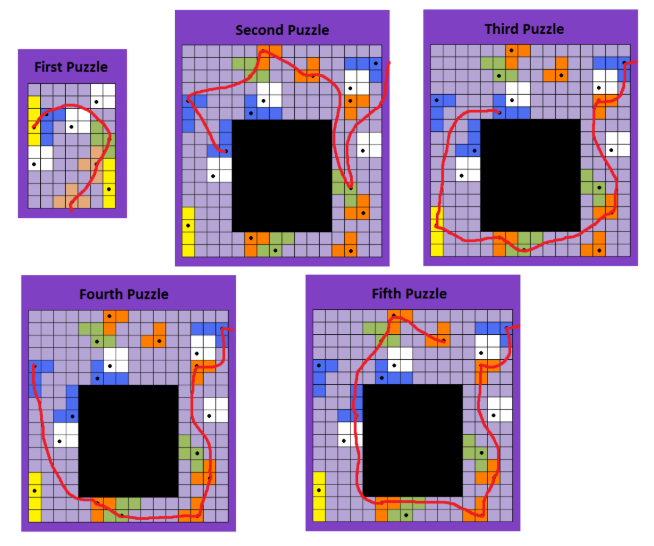
\includegraphics[scale=.9]{graphics/zanarkandpuzzles}
\begin{enumerate}[resume]
	\item After the fifth puzzle, take the Besaid Sphere and place it into the fifth pedestal and push it in
	\item \cs, run into the large room
\end{enumerate}
\begin{battle}[52000]{Spectral Keeper}
\begin{itemize}
	\summon{\bahamut}
	\bahamutf Attack
\end{itemize}
\end{battle}
\begin{spheregrid}
\begin{itemize}
	\item \textit{If you had 4 \textbf{Return Spheres}}: Agi+3, Str+2
	\item \yuna\ should have 70 Str and 35 Agi. If short, then the key Str Nodes are near \tidus's Armor Break and the end of \wakka's grid, and Agi is near \lulu\ (+8), \rikku\ (+3) and \wakka (+3 near Mag+3). If you need more Return Spheres to do these, then you can attack Sinspawn Genesis for an extra one, though it costs 26 seconds
\end{itemize}
\end{spheregrid}
\begin{enumerate}[resume]
	\item \save, Run up, \sd, walk up to Yunalesca's room, \sd
\end{enumerate}
\begin{battle}[132000]{Yunalesca}
\begin{itemize}
	\summon{\bahamut}
	\bahamutf Attack
\end{itemize}
Check for any weapon drops with \textbf{Zombie Strike}
\end{battle}
\begin{enumerate}[resume]
	\item \sd, leave room, walk down steps, \sd, go down on the next screens, \save, go up the lift, walk out of the cloister of trials, walk down the steps, walk down, \sd during \cs+\skippablefmv
\end{enumerate}
\chapter{Airship}
\begin{enumerate}
	\item \sd, walk out of the cockpit past Rin, along the corridors to \yuna\ and \kimahri. \sd. Walk back to the cockpit, \sd. Talk to Cid to travel to Highbridge.
	\item Walk up to the Bevelle entrance, \sd. In the Fayth room, pick ``Defeat Yu Yevon''
	\item Walk up to Cid, travel to Sin, \sd. Go through the corridors to the outside of the airship, \sd, 3 \skippablefmv[2:10], \sd
\end{enumerate}
\begin{battle}[65000]{Sin Left Fin}
\begin{itemize}
	\summon{\bahamut}
	\bahamutf Impulse x2
\end{itemize}
\end{battle}
\begin{enumerate}[resume]
	\item \sd, \cs+\skippablefmv
\end{enumerate}
\begin{battle}[65000]{Sin Right Fin}
\begin{itemize}
	\summon{\bahamut}
	\bahamutf Impulse x2
\end{itemize}
\end{battle}
\begin{enumerate}[resume]
	\item \sd, \cs+\skippablefmv
\end{enumerate}
\begin{battle}[56000]{Sin Genais and Core}
\begin{itemize}
	\summon{\bahamut}
	\bahamutf Impulse
\end{itemize}
Check for any weapon drops with \textbf{Zombie Strike}
\end{battle}
\begin{enumerate}[resume]
	\item \sd, \skippablefmv
	\item Walk along the corridors to the outside of the ship, speak to \yuna. \cs[1:40], \sd\ \rikku\ dialogue. \skippablefmv. Go through the corridors, go outside again, \skippablefmv, \sd.
\end{enumerate}
\begin{battle}[140000]{Overdrive Sin}
\begin{itemize}
	\item \textit{If 0 \textbf{Return Spheres}:} Give \tidus\ a turn
	\summon{\bahamut}
	\bahamutf Impulse
	\bahamutf Attack x2
\end{itemize}
\end{battle}
\begin{enumerate}[resume]
	\item \skippablefmv[1:20], \sd
\end{enumerate}
\chapter{Inside Sin}
\begin{enumerate}
	\item \formation{\tidus}{\kimahri}{\auron}
	\item Walk along the path, flee from all encounters.
	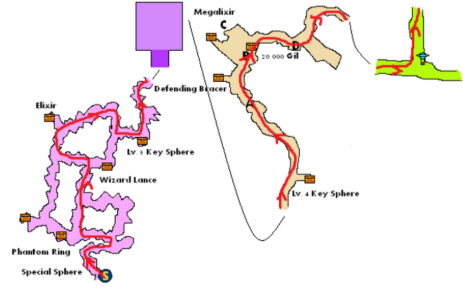
\includegraphics{graphics/sinpath}
	\item Before Seymour Omnis, \formation{\tidus}{\yuna}{\auron}
	\item Go up the steps, \sd
\end{enumerate}
\begin{battle}[80000]{Seymour Osmosis}
\begin{itemize}
	\yunaf Defend
	\tidusf Armor Break
	\item \textit{If Armor Break Hit:}
	\begin{itemize}
		\auronf Defend
		\summon{\bahamut}
		\bahamutf Attack
	\end{itemize}
	\item \textit{If Armor Break Missed:}
	\begin{itemize}
		\switch{\auronf}{\rikku}
		\rikkuf \od\ Mix Spherimorph Throwable + HiPot/MegaPot/XPot/Mega Phoenix
		\yunaf Cure Mortiphasm
		\tidusf Armor Break
		\summon{\bahamut}
		\bahamutf Attack
	\end{itemize}
\end{itemize}
\end{battle}
\begin{enumerate}
	\item \sd, walk north.
	\item \formation{\tidus}{\kimahri}{\auron}
	\item Make sure that \rikku's \od\ is charged
	\item Turn left onto the bridge, go onto the next screen. \save if needed.
	\item Complete the minigame, picking up the eggs and avoiding the crystals.
\end{enumerate}
\begin{spheregrid}
\begin{itemize}
	\item \textit{Bahamut Ending:}
	\begin{itemize}
		\item \textit{If you got 2/4 \textbf{Return Spheres}:}
		\begin{itemize}
			\yunaf Attribute Sphere \rikku's +3 Agi (hold L)
			\item Return Sphere ($\downarrow \downarrow \leftarrow \leftarrow$) or Friend Sphere ($\downarrow \leftarrow$) there
			\item Go down, picking up Agi+4, Spare Change, Agi+4
		\end{itemize}
		\item \textit{If you got 0 \textbf{Return Spheres}:}
		\begin{itemize}
			\yunaf Attribute Sphere \rikku's +3 Agi (hold L)
			\yunaf Go right, getting +4 Agi, +4 Agi
		\end{itemize}
		\tidusf If you didn't get a \textbf{Zombie Strike} weapon, then go back and learn Zombie Strike
		\rikkuf If no \od, use Skill Sphere to learn Armor Break
	\end{itemize}
	\item \textit{Quick Hit Ending:}
	\begin{itemize}
		\rikkuf Unlock Level 2 Key Sphere
		\item Move Up, Left
		\item Quick Hit
		\yunaf Use White Magic Sphere to learn Haste
		\yunaf Use Skill Sphere to learn Quick Hit
		\tidusf If you didn't get a \textbf{Zombie Strike} weapon, then go back and learn Zombie Strike
	\end{itemize}
\end{itemize}
\end{spheregrid}
\begin{enumerate}[resume]
	\item Walk up to Ject, \cs[4:30]
\end{enumerate}
\begin{battle}[180000]{Braska's Final Aeon}
\begin{itemize}
	\item \textit{Bahamut Ending:}
	\begin{itemize}
		\switch{\yuna}{\rikku}
		\rikkuf \od\ Mix Grenade + HP Sphere or Armor Break
		\tidusf Talk
		\switch{\auron}{\yuna}
		\summon{\bahamut}
		\bahamutf Attack
	\end{itemize}
	\item \textit{Quick Hit Ending:}
	\begin{itemize}
		\yunaf Haste \yuna
		\tidusf Talk
		\switch{\auron}{\rikku}
		\rikkuf \od\ Mix HP Sphere + Grenade for Chaos Grenade
		\yunaf Quick Hit
		\tidusf Talk
		\yunaf Quick Hits until out of MP
		\summon{\bahamut}
		\bahamutf Attack
	\end{itemize}
\end{itemize}
\end{battle}
\begin{enumerate}[resume]
	\item \cs+\skippablefmv[4:00]
\end{enumerate}
\begin{battle}{Possesed Aeons}
\begin{itemize}
	\item \textit{Bahamut Ending:}
	\begin{itemize}
		\item Spare Change as follows:
		\begin{itemize}
			\valeforf \num{20000} Gil
			\ifritf \num{30000} Gil
			\ixilonf \num{30000} Gil
			\bahamutf \num{40000} Gil
			\shivaf All Remaining Gil
		\end{itemize}
	\end{itemize}
	\item \textit{Quick Hit Ending:}
	\begin{itemize}
		\yunaf Elixer \yuna
		\item Option 1:
		\begin{itemize}
			\yunaf Quick Hit
			\yunaf Haste \yuna
			\yunaf Quick Hit
		\end{itemize}
		\item Option 2:
		\begin{itemize}
			\valeforf Waterga
			\ifritf Waterga
			\shivaf Waterga
			\bahamutf Waterga x2
			\ixilonf Switch Weapon to Mage's Staff
			\tidusf Defend
			\yunaf Waterga
		\end{itemize}
	\end{itemize}
\end{itemize}
\end{battle}
\begin{enumerate}[resume]
	\item \cs[1:40]
\end{enumerate}
\begin{battle}[99999]{Yu Yevon}
\begin{itemize}
	\item Anyone: Zombie Attack
	\item Anyone: Throw Phoenix Down
\end{itemize}
\end{battle}

	
\end{multicols}

\end{document}
